En Joan troba entre els papers del seu avi un esbós com el de la figura adjunta, on es descriu un terreny de
regadiu que ha deixat en herència al seu pare.
\begin{center}
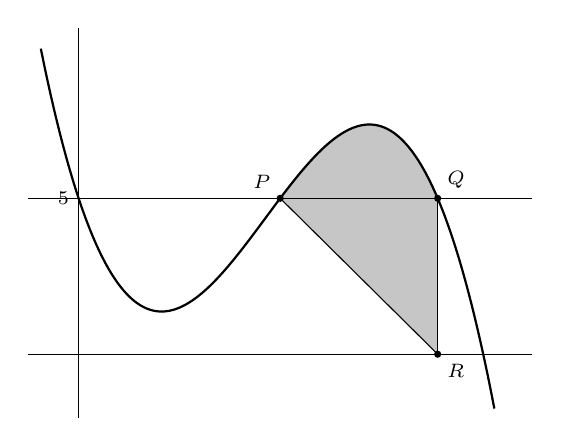
\begin{tikzpicture}[x=1.6cm,y=0.9cm]
  \fill[gray!45] (1.6,2.2) -- plot[domain=1.6:2.85,samples=60,smooth] (\x,{2.2-1.176*(\x)*((\x)-1.6)*((\x)-2.85)})
    -- (2.85,0) -- cycle;
  \draw (-0.4,0) -- (3.6,0);
  \draw (0,-0.9) -- (0,4.6);
  \draw (-0.4,2.2) -- (3.6,2.2);
  \draw (1.6,2.2) -- (2.85,0);
  \draw (2.85,2.2) -- (2.85,0);
  \draw[\colorgrafica,thick,domain=-0.3:3.3,samples=100,smooth] plot (\x,{2.2-1.176*(\x)*((\x)-1.6)*((\x)-2.85)});
  \node[left,font=\scriptsize] at (0,2.2) {$5$};
  \fill (1.6,2.2) circle (1.3pt);  \node[above left,font=\scriptsize] at (1.6,2.2) {$P$};
  \fill (2.85,2.2) circle (1.3pt); \node[above right,font=\scriptsize] at (2.85,2.2) {$Q$};
  \fill (2.85,0) circle (1.3pt);   \node[below right,font=\scriptsize] at (2.85,0) {$R$};
\end{tikzpicture}
\end{center}
La corba de la gràfica és $y=f(x)$, amb $f(x)=-x^3+7x^2-6x+5$.

\begin{apartats}

\apartat{1,25}
A partir de l'expressió de $f(x)$, calculeu les coordenades dels punts $P$, $Q$ i $R$ indicats a la figura.
Calculeu també l'equació de la recta $PR$.

\begin{solucio}
Tal com es veu al dibuix, les abscisses dels punts $(0,5)$, $P$ i $Q$ són les tres solucions de l'equació
$f(x)=5$:
\[
-x^3+7x^2-6x+5=5\;\rightarrow\;x\left(-x^2+7x-6\right)=0\;\rightarrow\;x=0,\quad
x=\frac{-7\pm\sqrt{49-24}}{-2}=1,\ 6 .
\]
Per tant, les coordenades dels punts demanats són $P=(1,5)$, $Q=(6,5)$ i $R=(6,0)$. Ara, la recta $r$ que passa
pels punts $P=(1,5)$ i $R=(6,0)$ té pendent $m=\frac{0-5}{6-1}=-1$; per tant, és $y=-x+n$ i, com que passa pel
punt $R=(6,0)$, tenim que $n=6$: es tracta de la recta $y=-x+6$.

\textit{Pauta oficial:} 0,25 per plantejar bé l'equació, 0,25 per resoldre-la, 0,25 per donar les coordenades
dels tres punts i 0,5 per l'equació de la recta.
\end{solucio}

\apartat{1,25}
Calculeu la superfície del terreny.

\begin{solucio}
La superfície del terreny serà la integral definida entre els punts d'abscissa $x=1$ i $x=6$ de la funció
$f(x)$ menys la recta:
\begin{align*}
A&=\int_1^6\bigl(f(x)-r(x)\bigr)\,dx=\int_1^6\Bigl(\left(-x^3+7x^2-6x+5\right)-(-x+6)\Bigr)\,dx
=\int_1^6\left(-x^3+7x^2-5x-1\right)dx\\
&=\left[-\frac{x^4}{4}+\frac73x^3-\frac52x^2-x\right]_1^6\\
&=\left(-\frac{6^4}{4}+\frac73\,6^3-\frac52\,6^2-6\right)-\left(-\frac14+\frac73-\frac52-1\right)
=\frac{1025}{12}=85{,}416\ldots\ \text{u}^2 .
\end{align*}
Alternativament, es pot integrar només $f(x)$ entre 1 i 6, i restar-hi el triangle inferior, que no és del
terreny:
\begin{align*}
A&=\int_1^6f(x)\,dx-\frac{5\cdot5}{2}=\int_1^6\left(-x^3+7x^2-6x+5\right)dx-\frac{25}{2}
=\left[-\frac{x^4}{4}+\frac73x^3-3x^2+5x\right]_1^6-\frac{25}{2}\\
&=\frac{1175}{12}-\frac{25}{2}=85{,}416\ldots\ \text{u}^2 .
\end{align*}

\textit{Pauta oficial:} 0,5 pel plantejament de la integral correcta i 0,75 per fer-ne el càlcul. Compteu bé
qualsevol de les maneres de fer-ho, si són correctes i estan ben explicades.
\end{solucio}

\end{apartats}
